\documentclass[10pt,a4paper]{article}
\usepackage[utf8]{inputenc}
\usepackage[T1]{fontenc}
\usepackage{mathptmx}
\usepackage[top=52mm,bottom=43mm,left=40mm,right=40mm]{geometry}
\usepackage{graphicx}
\usepackage{booktabs}
\usepackage{tabularx}
\usepackage{float}
\usepackage{microtype}
\usepackage{caption}
\usepackage[hidelinks]{hyperref}
\usepackage[numbers,sort&compress]{natbib}
\usepackage{titlesec}
\usepackage{parskip}
\usepackage{xcolor}

% LNCS-style formatting
\pagestyle{empty}
\setlength{\parindent}{0pt}
\setlength{\parskip}{5pt}

\titleformat{\section}{\normalsize\bfseries}{\thesection}{1em}{}
\titleformat{\subsection}{\normalsize\itshape}{\thesubsection}{1em}{}
\titlespacing*{\section}{0pt}{10pt}{4pt}
\titlespacing*{\subsection}{0pt}{8pt}{3pt}

\captionsetup{font=small,labelfont=bf,skip=4pt}

\begin{document}

% ── Title block ───────────────────────────────────────────────────────────────
\begin{center}
{\Large\bfseries
Automatic Detection of Lexical Ambiguity Patterns\\[4pt]
in Functional Requirements: An Exploratory Study\\[4pt]
in the Meat Traceability Domain\par}

\vspace{10pt}

{\normalsize
Ariel Omar Castro Baja\~{n}a,
Kleber Obed Crespo Espinoza,
Edhu Xavier Gamarra Araujo,\\
Carlos Andr\'{e}s P\'{e}rez Ruiz, and
Erick Jahir Quintero Gende\par}

\vspace{4pt}

{\small\itshape
Facultad de Ciencias de la Computaci\'{o}n,
Universidad T\'{e}cnica Estatal de Quevedo (UTEQ),
Quevedo, Los R\'{i}os, Ecuador\\
\texttt{\{acastrob, kcrespoe, egamarraa, cperezr3, equinterog\}@uteq.edu.ec}\par}
\end{center}

\vspace{8pt}

% ── Abstract ──────────────────────────────────────────────────────────────────
\noindent\textbf{Abstract.}
\textbf{Context.} Functional requirements (FRs) written in natural language are
prone to lexical ambiguity, propagating defects to later development phases.
Automated detectors for Spanish-language FR corpora in Latin~American
agroindustrial domains are scarce.
\textbf{Objective.} To characterise the lexical-syntactic ambiguity patterns
present in the 27~FRs of CarniCore---a real-world meat distribution management
system in Ecuador---using a rule-based automatic detector.
\textbf{Method.} A deterministic Python detector covering three categories
(vague quantifiers, multiple conjunctions, and agentless passive voice) was
applied to the complete verbatim FR corpus of ERS/SRS~v2.0.
The study protocol was pre-registered at OSF prior to data
collection~\cite{osf2026carnicore}.
\textbf{Results.} One out of 27~FRs (3.7\%) triggered the detector: RF-27
activated the vague-quantifier category through the term
\textit{correspondiente}.
The remaining 26~FRs (96.3\%) showed no lexical-syntactic patterns.
\textbf{Conclusions.} Rule-based detectors act as a low-cost first filter for FR
quality; a near-zero rate shifts residual ambiguity risk to the semantic and
pragmatic levels. Replication package:
\url{https://doi.org/10.5281/zenodo.22225854}.

\smallskip
\noindent\textbf{Keywords:}
Requirements ambiguity $\cdot$
Automatic detection $\cdot$
Functional requirements $\cdot$
Empirical study $\cdot$
Ecuador $\cdot$
Meat traceability

\vspace{6pt}
\hrule
\vspace{6pt}

% ═══════════════════════════════════════════════════════════════════════════════
\section{Introduction}
\label{sec:intro}

Meat distribution companies in Ecuador manage animal traceability manually,
generating inconsistencies that hinder compliance with sanitary regulations
imposed by Agrocalidad. CarniCore digitalises that process through 27 functional
requirements written in natural-language Spanish, covering supplier registration,
animal intake, cold-chain monitoring, weight ticketing, and QR-based
traceability~\cite{iso29148}.
The lexical quality of those FRs determines downstream quality: ambiguous
requirements propagate defects to design, testing, and
maintenance~\cite{mendez2017naming}.

Automatic ambiguity detection has been studied mainly for English-language
corpora~\cite{ferrari2019nlp,femmer2017smells,gervasi2017ambiguity}.
Cheng et al.~\cite{cheng2026genai} identify this geographic and linguistic gap
in their systematic review of 100+ studies: no work targets Spanish FR corpora
from Latin~American agroindustrial domains. Arora et al.~\cite{arora2024genai}
confirm that most detectors were validated on software products from high-income
countries, limiting generalisability.

This work makes three contributions:
(1)~an open-source rule-based detector of lexical-syntactic ambiguity patterns
in Spanish;
(2)~its application to a real corpus of 27~FRs of a meat traceability system,
yielding the first documented characterisation of this domain in the requirements
ambiguity literature; and
(3)~a FAIR replication package with anonymised data and reproducible scripts.

\noindent\textbf{RQ1.} What proportion of CarniCore's FRs triggers at least one
lexical-syntactic ambiguity pattern?\\
\noindent\textbf{RQ2.} Which ambiguity categories are most frequent in the corpus?

% ═══════════════════════════════════════════════════════════════════════════════
\section{Related Work}
\label{sec:related}

Table~\ref{tab:related} summarises the six most relevant studies.
Ferrari and Esuli~\cite{ferrari2019nlp} achieved $F_1\!\geq\!0.70$ using NLP
cross-domain models for English. Femmer et al.~\cite{femmer2017smells} introduced
12 requirements smells detectable by rules, applied to industrial German-language
documents. Gervasi et al.~\cite{gervasi2017ambiguity} provided a taxonomic review
but no applied detector. Fischbach et al.~\cite{fischbach2023acceptance} combined
NLP and LLMs to extract acceptance tests. Unlike all prior work, this study
targets Spanish, an unexplored agroindustrial domain, and makes the corpus and
detector fully reproducible under CC~BY~4.0.

\begin{table}[H]
\centering
\caption{Comparison with related work on FR ambiguity detection}
\label{tab:related}
\small
\begin{tabular}{lllp{3.2cm}p{3.0cm}}
\toprule
\textbf{Reference} & \textbf{Year} & \textbf{Lang.} & \textbf{Method} & \textbf{Key difference} \\
\midrule
Ferrari \& Esuli~\cite{ferrari2019nlp}     & 2019 & EN & NLP cross-domain & No Spanish, no agro \\
Femmer et al.~\cite{femmer2017smells}      & 2017 & DE/EN & Rules (smells) & No Spanish corpus \\
Gervasi et al.~\cite{gervasi2017ambiguity} & 2017 & EN & Taxonomy review & No applied detector \\
Fischbach et al.~\cite{fischbach2023acceptance} & 2023 & EN & NLP + LLM & Acceptance tests only \\
Cheng et al.~\cite{cheng2026genai}         & 2026 & EN & SLR (100+ studies) & No applied detector \\
\textbf{This work}                         & \textbf{2026} & \textbf{ES} & \textbf{Rules} & \textbf{Spanish, meat, FAIR} \\
\bottomrule
\end{tabular}
\end{table}

% ═══════════════════════════════════════════════════════════════════════════════
\section{Methodology}
\label{sec:method}

\subsection{Study Design and PICOC}

We conducted a descriptive exploratory study~\cite{runeson2009}:
\textbf{Population}---27 verbatim FRs from ERS/SRS~v2.0 of CarniCore (Pucayacu,
La~Man\'{a}, Ecuador);
\textbf{Intervention}---rule-based automatic detector;
\textbf{Comparison}---none (single-arm; expert panel deferred to future work,
see DEV-01);
\textbf{Outcome}---proportion of FRs triggering $\geq\!1$ category;
\textbf{Context}---4th-year undergraduate project, UTEQ, 2026.

\subsection{Detector Design}

The detector (\texttt{detector\_ambiguedad.py}) applies three lexical-syntactic
rules over the verbatim Spanish text of each FR:

\textbf{C1 -- Vague quantifiers.} Matches terms whose referent is
unverifiable without additional context: \textit{algunos}, \textit{varios},
\textit{adecuado}, \textit{suficiente}, \textit{r\'{a}pido},
\textit{correspondiente(s)}, \textit{oportuno}, \textit{apropiado},
\textit{razonable}, among others.

\textbf{C2 -- Multiple conjunctions.} Flags FRs containing $>\!3$ connectors
(\textit{y}/\textit{o}) or $>\!2$ modal verbs, following Femmer et al.'s
compound-sentence smell~\cite{femmer2017smells}.

\textbf{C3 -- Agentless passive voice.} Detects participial constructions
(\textit{ser\'{a} generado}, \textit{deber\'{a} ser registrado}) without an
explicit actor, violating verifiability~\cite{iso29148}.

A FR receives \texttt{ambiguo\_detector\,=\,1} if it activates $\geq\!1$
category. The analysis is fully deterministic and reproducible from the raw
corpus file~\cite{zenodo2026carnicore}.

\subsection{Participants and Data Collection}

Field work was conducted in two rounds (July--August 2026) under the
LOPDP~\cite{lopd2021}. Five semi-structured interviews were conducted with four
stakeholder profiles: warehouse manager ($n\!=\!2$), butcher/dispatcher
($n\!=\!1$), reception and weighing operator ($n\!=\!1$), and owner ($n\!=\!1$).
A questionnaire was applied to 31~respondents across six operational roles
(weighing and labelling: 7; supplier reception: 7; sales: 6; butchering: 5;
supervision: 3; storage: 2). Five walkthrough sessions validated the FR
specification. Identifiable material is stored in an AES-256 encrypted container
accessible only to the supervising faculty member; only anonymised data appear
in the public package~\cite{zenodo2026carnicore}.

\subsection{Protocol Registration and Deviations}

The protocol was pre-registered at OSF on 02/08/2026, before data collection,
following Nosek et al.~\cite{nosek2018prereg}.
Two deviations are documented:
\textbf{DEV-01}---the comparative phase (precision, recall, $F_1$,
Cohen's~$\kappa$ against an expert panel) was not executed due to the
unavailability of independent evaluators; no metrics are imputed.
\textbf{DEV-02}---the corpus was extended from 25 to 27~FRs after CCB approval
of RF-26 and RF-27 post-registration.

% ═══════════════════════════════════════════════════════════════════════════════
\section{Results}
\label{sec:results}

\subsection{RQ1: Proportion of Flagged FRs}

Table~\ref{tab:results} shows the output of \texttt{run\_all.sh} over the
27-FR corpus.
One FR out of 27 (3.7\%) was flagged by the detector.

\begin{table}[H]
\centering
\caption{Detector results across the 27 FRs of CarniCore}
\label{tab:results}
\small
\begin{tabular}{lcc}
\toprule
\textbf{Category} & \textbf{FRs triggered} & \textbf{Percentage} \\
\midrule
C1 -- Vague quantifier        & 1 / 27 & 3.7\% \\
C2 -- Multiple conjunctions   & 0 / 27 & 0.0\% \\
C3 -- Agentless passive voice & 0 / 27 & 0.0\% \\
\midrule
\textbf{Any category (flagged)} & \textbf{1 / 27} & \textbf{3.7\%} \\
\bottomrule
\end{tabular}
\end{table}

The sole flagged requirement is RF-27:

\begin{quote}
\small\itshape
``El sistema deber\'{a} permitir \ldots\ mostrando los totales
\textbf{correspondientes} a ese proveedor en el rango de fechas seleccionado.''
\end{quote}

The term \textit{correspondientes} is a vague quantifier: it does not specify
which totals are included (sales only? with returns? before or after tax?),
making RF-27 unverifiable without stakeholder clarification~\cite{pohl2010}.

\subsection{RQ2: Category Distribution}

Figure~\ref{fig:categories} shows the distribution of activated categories.
Figure~\ref{fig:status} maps detection status per individual FR.
Categories C2 and C3 recorded zero activations, indicating consistent use of
simple conjunctions and active voice (\textit{El sistema deber\'{a}\ldots})
across the corpus.

\begin{figure}[H]
\centering
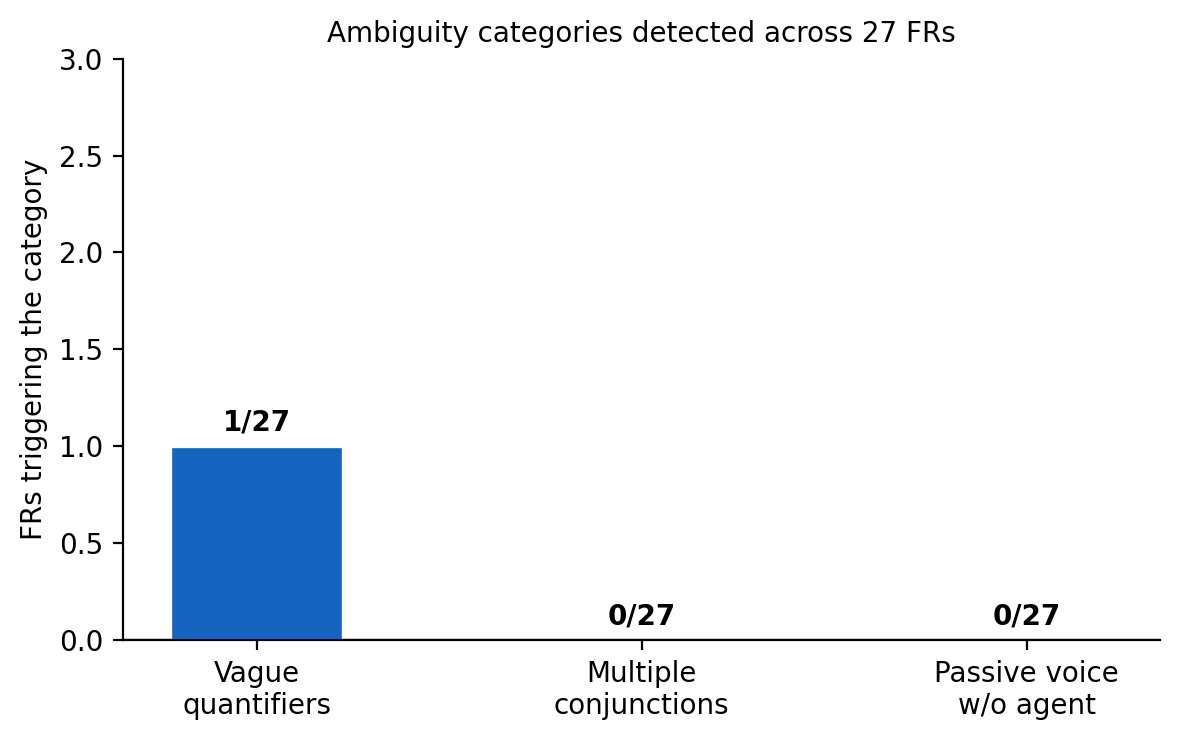
\includegraphics[width=0.72\linewidth]{figuras/fig1_categories.png}
\caption{Distribution of detected ambiguity categories ($n\!=\!27$ FRs).
         Generated by \texttt{run\_all.sh} from \texttt{clasificaciones\_detector.csv}.}
\label{fig:categories}
\end{figure}

\begin{figure}[H]
\centering
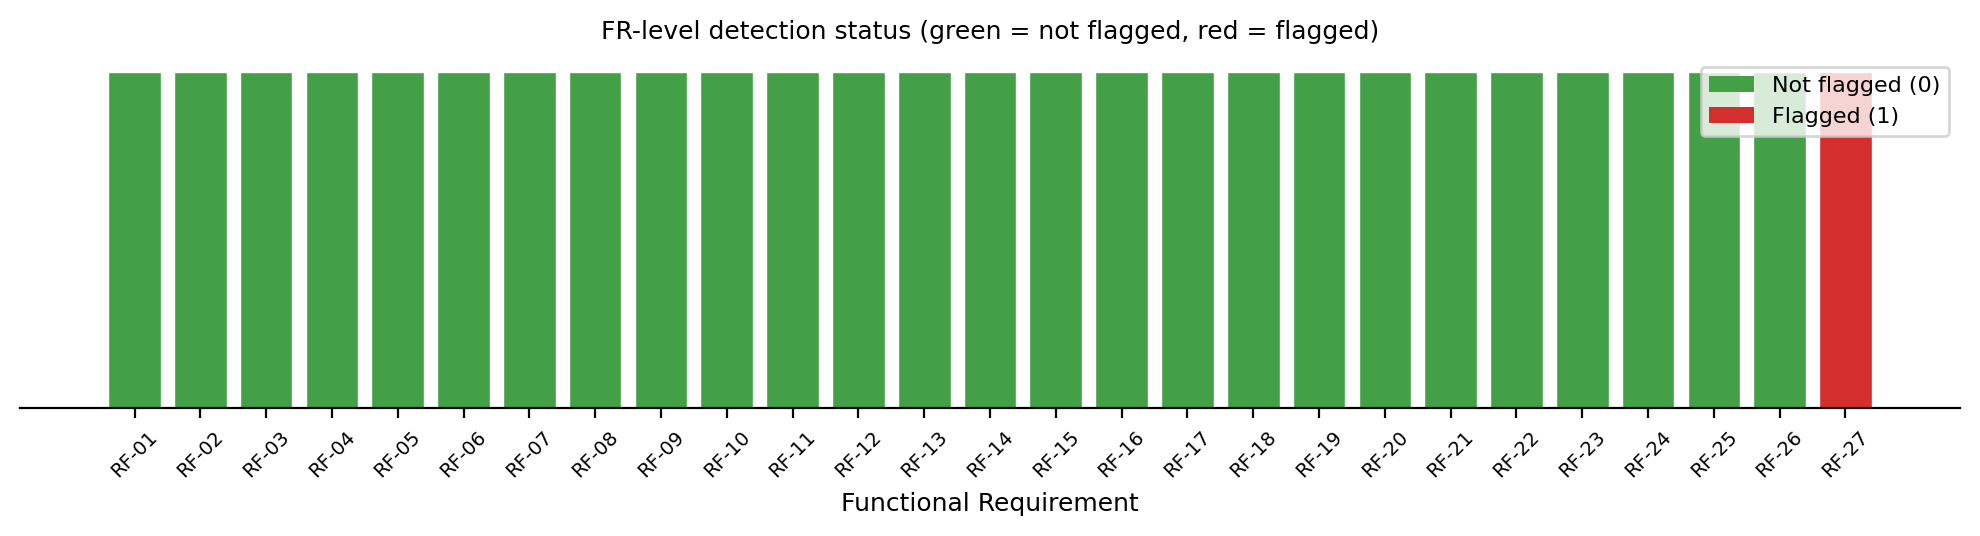
\includegraphics[width=\linewidth]{figuras/fig2_fr_status.png}
\caption{FR-level detection status: green = not flagged (26/27);
         red = flagged (1/27, RF-27).}
\label{fig:status}
\end{figure}

% ═══════════════════════════════════════════════════════════════════════════════
\section{Discussion}
\label{sec:discussion}

\subsection{Implications for Research}

The near-zero detection rate suggests that the active-voice template combined
with explicit quantitative thresholds (``m\'{a}ximo 3 d\'{i}as para pollo'')
acts as an effective embedded lexical-quality control, consistent with Ferrari
and Esuli~\cite{ferrari2019nlp}, who report lower ambiguity rates in corpora
produced with structured elicitation protocols.
For Spanish-language corpora produced with similar templates, semantic and
pragmatic ambiguity are likely more prevalent quality risks than lexical ambiguity.

\subsection{Implications for Practice}

Two actionable insights emerge. First, enforcing an active-voice template with
mandatory thresholds at writing time reduces lexical ambiguity without post-hoc
tooling. Second, the sole flagged term (\textit{correspondientes} in RF-27) is
remediable: replacing it with ``los totales de ventas, compras y p\'{e}rdidas
netas antes de devoluciones'' removes the ambiguity without changing intent.

\subsection{Surprising Findings}

The complete absence of C2 and C3 across 27~FRs is counterintuitive given the
complexity of some requirements (e.g., RF-08 specifies four shelf-life limits in
one sentence; RF-21 describes an offline-sync mechanism). We attribute this to
the modal anchor \textit{deber\'{a} permitir}, which naturally forces active
voice and limits connector proliferation.

% ═══════════════════════════════════════════════════════════════════════════════
\section{Threats to Validity}
\label{sec:threats}

Following Wohlin et al.~\cite{wohlin2012}:

\noindent\textbf{Internal.} The analysis is deterministic and reproducible;
no selection bias (complete census). Threat: regex coverage---terms absent
from the pattern list would not be detected.

\noindent\textbf{Construct.} The detector covers only lexical-syntactic ambiguity;
semantic and pragmatic ambiguity require expert reading.

\noindent\textbf{External.} 27~FRs from one system in one country; generalisation
requires replication. The published dataset enables this~\cite{zenodo2026carnicore}.

\noindent\textbf{Conclusion.} Without an expert panel (DEV-01), precision and
recall cannot be computed. Results are descriptive only.

% ═══════════════════════════════════════════════════════════════════════════════
\section{Conclusions and Future Work}
\label{sec:conclusions}

\textbf{RQ1:} 1 out of 27 FRs (3.7\%) triggered the detector, well below rates
reported for unstructured English corpora.
\textbf{RQ2:} Only the vague-quantifier category was activated (RF-27,
\textit{correspondientes}); multiple conjunctions and agentless passive voice
recorded zero activations.
Structured active-voice templates with explicit thresholds appear to be effective
lexical quality controls for Spanish-language FRs in agroindustrial domains.

\noindent\textbf{Future work:}
(1)~Execute with $\geq\!3$ expert evaluators (completing DEV-01).
(2)~Extend to other Spanish-language FR corpora.
(3)~Compare with LLM-based detection on the same published corpus.

% ── Data availability ─────────────────────────────────────────────────────────
\section*{Data Availability}
Replication package (anonymised transcripts, questionnaire responses [$n\!=\!31$],
labelled RF corpus in JSON, traceability matrix, LLM prompts, Python scripts):
\url{https://doi.org/10.5281/zenodo.22225854} (CC~BY~4.0).
Pre-registration: \url{https://osf.io/wud69}.
Repository: \url{https://github.com/EdhuXav/CarniCore_Proyecto_ISR401}.

% ── AI declaration ────────────────────────────────────────────────────────────
\section*{Use of AI-assisted Technologies}
Claude (Anthropic, claude-sonnet-4-6) was used for paragraph editing and
\LaTeX{} formatting. All empirical results and conclusions are the authors'
own work validated against primary evidence.

% ── Acknowledgements ──────────────────────────────────────────────────────────
\section*{Acknowledgements}
The authors thank the staff of Distribuidora C\'{a}rnicos Pucayacu for their
participation. Supervised by PhD.\ Guerrero Ulloa Gleiston
Cic\'{e}r\'{o}n, UTEQ. ISR-401 course, 2026--2027~PPA.

% ── References ────────────────────────────────────────────────────────────────
\bibliographystyle{splncs04}
\bibliography{referencias}

\end{document}
